%% Template for SDP report, adapted from mlp_cw2_template, 2018. 

%% Based on  LaTeX template for ICML 2017 - example_paper.tex at 
%%  https://2017.icml.cc/Conferences/2017/StyleAuthorInstructions

\documentclass{article}
\usepackage[T1]{fontenc}
\usepackage{amssymb,amsmath}
\usepackage{txfonts}
\usepackage{microtype}
\usepackage{xspace}
\xspaceaddexceptions{\%}

% Lists with less spacing between items
\usepackage{paralist}

% For figures
\usepackage{graphicx}
\usepackage{subfig} 

% For citations
\usepackage{natbib}

% For algorithms
\usepackage{algorithm}
\usepackage{algorithmic}

% the hyperref package is used to produce hyperlinks in the
% resulting PDF.  If this breaks your system, please commend out the
% following usepackage line and replace \usepackage{mlp2017} with
% \usepackage[nohyperref]{mlp2017} below.
\usepackage{hyperref}
\usepackage{url}
\urlstyle{same}

% Packages hyperref and algorithmic misbehave sometimes.  We can fix
% this with the following command.
\newcommand{\theHalgorithm}{\arabic{algorithm}}


% Set up MLP coursework style (based on ICML style)
\usepackage{mlp2018}
\mlptitlerunning{SDP Demo \demoNumber  Group (\groupNumber)}
\bibliographystyle{icml2017}


\DeclareMathOperator{\softmax}{softmax}
\DeclareMathOperator{\sigmoid}{sigmoid}
\DeclareMathOperator{\sgn}{sgn}
\DeclareMathOperator{\relu}{relu}
\DeclareMathOperator{\lrelu}{lrelu}
\DeclareMathOperator{\elu}{elu}
\DeclareMathOperator{\selu}{selu}
\DeclareMathOperator{\maxout}{maxout}







%% You probably do not need to change anything above this comment

%% REPLACE the details in the following commands with your details
\setGroupNumber{15}
\setGroupName{Detroit}
\setProductName{Tadashi}
\setLogoFileName{figs/sdp_logo_placeholder.png}

\begin{document} 

\makeSDPTitle{Project Plan}

% Previous MLP Style Title Layout working. 
% \twocolumn[
    % \mlptitle{\productName: SDP Demo \demoNumber}
    % \centerline{Group \groupNumber: \groupName}
% ]

\begin{abstract}
  We propose an assistive healthcare robot, {\it Tadashi}, to automate simple tasks within a care home or supported living environment and allow caregivers to spend more time caring for their patients.
  {\it Tadashi} will automate three key tasks in the caregiver's day. Firstly, waking a patient up at a time specified by the caregiver, by coming into their room and speaking to them. Secondly, checking the patient is taking the correct medication at the correct time, by coming into their room; taking a picture of their medication; and having the caregiver verify it is the correct medication. Thirdly, checking on the welfare of the patient while the caregiver is occupied elsewhere, by coming to their room and asking the patient if they are okay and if they need a caregiver to attend to them. 
\end{abstract} 

\section{Goal description}
Caregivers are overworked: they spend a large amount of time on menial tasks, limiting the amount of time they can spend caring for patients. Our assistive healthcare robot allows caregivers to automate certain menial and administrative tasks, allowing them to spend less time on the menial work, and more time doing what matters: caring for their patients. 

\subsection{Relevance of the system}
\subsubsection{The problem space}
Tadashi is designed to tackle two problems facing caregivers in assisted living situations:
\begin{enumerate}
\item High caregiver:patient ratios, meaning caregivers have little time to dedicate per patient;
\item High administrative loads on caregivers, meaning they must spend more time on administration and menial tasks and less on caring for their patients directly.
\end{enumerate}

There is no national guidance on staffing levels and caregiver:patient ratios in care homes \cite{rcnstaffingadvice}, but research shows that in care homes there is an average ratio of 18 patients per registered nurse during the day, and 26 patients at night \cite{rcnstaffingguidance}.

With this many patients to take care of, nurses struggle to get the time they need with patients. In a 2017 survey on the impact of high nurse:patient ratios \cite{unison}:
\begin{itemize}
\item 63.2\% of nurses said that comforting or talking to patients was rushed, unfinished, not done to an acceptable standard, or missed entirely. 
\item 54\% said medication administration errors happened often or sometimes; only 54\% said that administering medication on time was done to acceptable standards.
\end{itemize}

Equally, a 2013 survey showed that nurses spend almost 1/5 of their day on administrative tasks; and only 20\% are satisfied with how they spend their time --- preferring to spend less time on admin and more time on direct care \cite{rcnpol}.

These problems will only get worse in the future. It is estimated that by 2035, up to 190,000 people more people aged 65 years or above will require some level of care, and increase of 86\% from today \cite{lancet}. Meanwhile, ongoing staffing issues in the NHS mean that in 10 years time the NHS will have a shortfall of 108,000 nurses \cite{nuffield}. This combination of factors will drive demand for innovative solutions --- including assistive technology like Tadashi. 

\subsubsection{Compliance with existing guidelines}
NICE healthcare guidelines \cite{niceguidance} advise care home providers to consider two key aspects in administering medication:
\begin{enumerate}
\item The 6 R's of administration: the right resident, the right medicine, the right route, the right dose, the right time, and the resident's right to refuse. 
\item Ensuring a record of administration is made as soon as possible. 
\end{enumerate}

Tadashi helps caregivers with these key aspects:
\begin{enumerate}
  \item Using the schedule specified by the caregiver, Tadashi ensures the right resident receives medication at the right time.
  \item By having the caregiver confirm the medication via the picture, Takashi ensures that the right medication is being taken at the right dose.
  \item By taking a picture of the medication and storing proof of the nurse's confirmation, Tadashi ensures a record of administration is made as soon as possible. 
\end{enumerate}

\subsubsection{Existing solutions}
The most relevant existing solution to the problems we have identified is the work of Fraunhofer IPA on service robots in residential care facilities. As part of the WiMi-Care project, they implemented and tested Care-O-bot 3, a `robot butler' that tracks residents' hydration and brings them water if they have not drunk enough. The goal of this project was to automate certain service-related tasks in order to relieve pressure on care staff. \cite{fraunhofer}

The key takeaways from this work that we will take into account in our project:
\begin{itemize}
\item Patient feedback to the robot was positive: ``inhabitants  understood  the  idea  of  a  robot  supporting  the  staff  without replacing them and showed no fear to interact with the machine'' \cite{springer}. 
\item Adding speech output to address patients by name helped to improve perceptions of the robot and compliance with drinking the water it offered \cite{ieee}. 
\item Staff reaced positively to the introduction of the robot: ``The overall reaction from the personnel (...) was very positive'' (ibid). 
\end{itemize}

\subsection{High-level description} 


\section{Task planning}
In this section you must provide a detailed plan of the tasks to be completed to achieve your goals. The plan must comprise two levels: first a few milestones that correspond to major achievements in the project, then a detailed list of atomic tasks that must be achieved.

\subsection{Milestones} 
From the user stories, you should extract the main technical subgoals, i.e., what you need to accomplish to get to the desired final result. For each subgoal you should provide an explicit milestone that states what you should have achieved, by what date, and what evidence you will present to show you have achieved it (e.g. a demonstration of the feature to the experts).


\subsection{Task decomposition} 
Each milestone should then be decomposed into a set of ``atomic'' tasks, taking no more than 20 hours each. Each task should be given a name, a one-sentence-long description, and an estimated time for completion.


You can summarize the tasks in a table, (for instance, table~\ref{tab:sample-table}, using the \verb+table+ environment).

\begin{table*}[h]
\vskip 3mm
\begin{center}
\begin{small}
\begin{sc}
\begin{tabular}{lcccr}
\hline
\abovespace\belowspace
Task Name & Milestone  & Estimated time & Dependency &  Rough description \\
\hline
\abovespace
Task 1 & Milestone 1    & 0.5 Days & - & Description 1 \\
Task 2 & Milestone 1    & 1 Day  & Task 1 & Description 2 \\
Task 3 & Milestone 2    & 2 Days & Milestone 1 & Description 3 
\belowspace
\end{tabular}
\end{sc}
\end{small}
\caption{Task decomposition for the system}
\label{tab:sample-table}
\end{center}
\vskip -3mm
\end{table*}

The report must include a Gantt chart, which should clearly identify any dependencies between the tasks. You may find it useful to make a revised version of your plan/gantt chart at key points in the project, in discussion with the experts. 

You can include the Gantt chart as a Latex figure (such as figure~\ref{fig:sample-fig}), use the \verb+\includegraphics+ environment to include an image (pdf, png, or jpg formats), ideally with informative labels added. 

To keep your folders clean, it is often a good idea to keep your images in a separate folder. In this example, we've put the figures in the \texttt{figs/} folder. To include images from different folders, give the relative path from this file. Example: \verb+\includegraphics{figs/image_filename}+.

\begin{figure}[tb]
\vskip 5mm
\begin{center}
\centerline{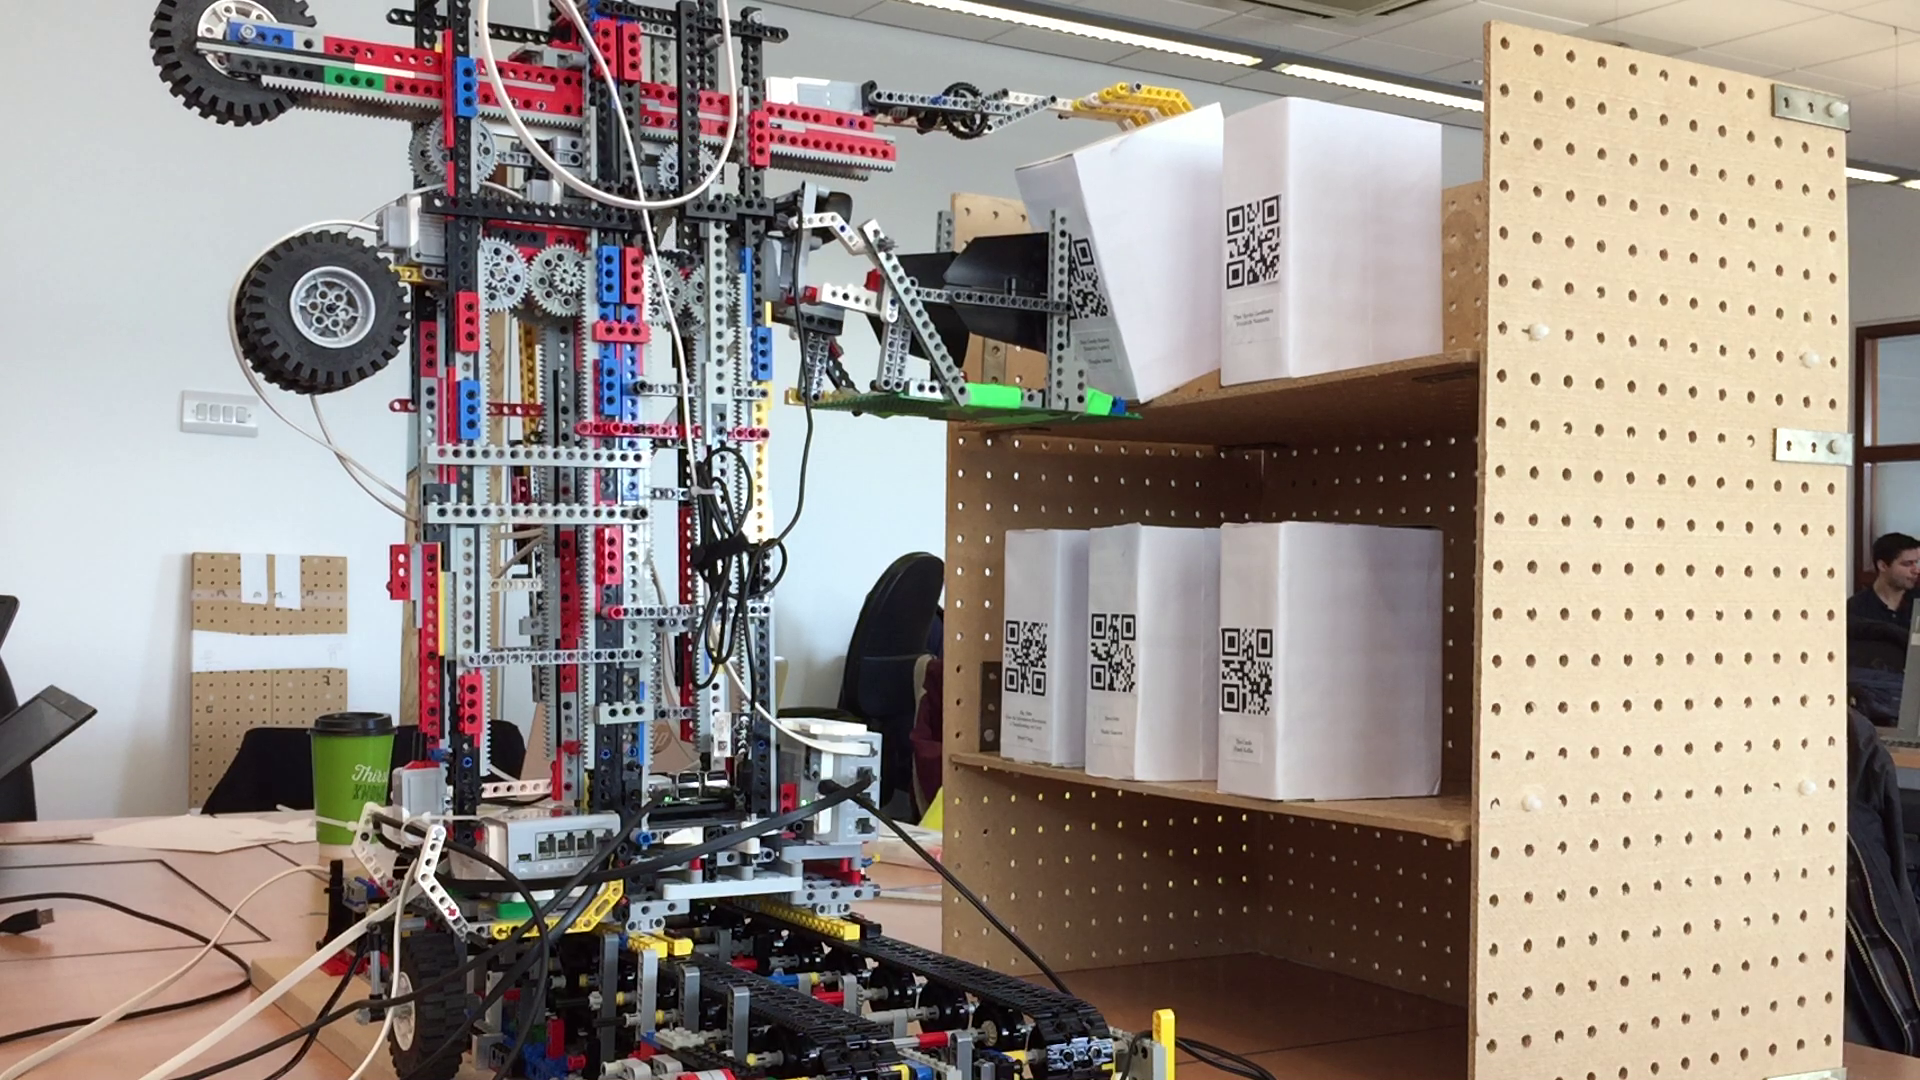
\includegraphics[width=\columnwidth]{figs/crane}}
\caption{Lego construction: highlight any salient features in the caption}
\label{fig:sample-fig}
\end{center}
\vskip -5mm
\end{figure} 


\subsection{Resource distribution}
The plan should explain how you will deploy your resources - 200 hours per group member over the semester - to achieve your goals. Note you should take into account time required by scheduled sessions (workshops, demo days, final presentations) and time used in planning and presenting (group meetings, report writing etc.). 

You should also list the resources you have in terms of skills, equipment, etc. The use of tables is also recommended for this section.

\subsection{Risk assessment} 
The report should also contain an assessment of the risks that you anticipate for the project, and contingency planning that you have done to guard against them. 

\section{Group organisation}
\begin{table}[]
  \begin{tabular}{lll}
    \hline
    Robot building & Robot coding & App development   \\
    \hline
    {\bf Jakub}          & {\bf Wojtek}       & {\bf Theo}              \\
    Luukas         & Ben          & Yuchen            \\
    Rebecca        & Errikos      & Ching Ling \\
    \hline
    Project management: & {\bf Michael} & \\
  \end{tabular}
  \caption{Team splits across the group. Names in bold are key points of contact.}
  \label{tab:group-split}
\end{table}

We will split the group into {\bf three core teams}: robot building, robot software, and app development (table~\ref{tab:group-split}). Each team has a team lead (in bold), responsible for co-ordinating with the other groups as necessary during the development process and holding responsibility for ensuring the group is tracking to its milestones.

The project manager (PM) holds overall responsibility for keeping the project on track: primarily through helping each team plan, execute, and validate its progress against milestones. The PM is also responsible for time management; writing up reports; and helping teams with any blockers they encounter in their work.

Structuring the teams in this manner allows us to use the {\it functional} organizational structure. This has particular benefits in allowing everyone within each team to focus on developing expertise in their area, as well as improving efficiency in communication within the team.

The disadvantage of using a functional structure is that it can make communication between teams difficult. To minimize this, we have decided a key point of contact (POC), in bold, for each team: POCs will communicate with each other and the PM on key issues and when cross-team collaboration is needed --- for example, in interfacing the robot hardware with the robot software. This eases communication between teams because it means there will only need to be four people meeting at once to represent all teams, rather than all ten group members needing to be present.

{\bf Each team will meet at a minimum once a week} to discuss their progress against their milestones; however, as demo days approach it will likely move to two or three times a week. Additionally the team POCs will meet once a week to make sure that any cross-team integration issues are handled, as well as to support each other if needed. 

{\bf Code-sharing} will be done exclusively through GitHub. Using version control more generally allows us to track our work over time and easily deal with any merge conflicts or other issues that may come up in doing distributed development. GitHub was chosen primarily because all members of the group are somewhat familiar with it, meaning there will be a shallower learning curve to complete our project using it. 

Using GitHub also allows us to do {\bf task allocation and progress sharing} using GitHub projects. We will follow a Kanban approach, separating tasks into ``to do'', ``in progress'', and ``done'', with one board per team. Using Kanban allows for team members to clearly see what tasks need to be done before the next demo; choose to begin working on tasks they feel they are suitable for; and to identify where there may be blockers within their work (ie. cards that are spending extended time in ``to do''). Additionally, making these boards public allows for other teams to see how work is progressing in the rest of the group. Progress updates will also be discussed in weekly team meetings on a granular level and more broadly in POC meetings.

{\bf Communication} will be done primarily through a dedicated Slack workspace, with separate channels for each team ({\tt robot-app}, {\tt robot-building}, {\tt robot-coding}, {\tt report-writing}, and {\tt general} for cross-team discussion). Using Slack allows us to integrate other apps, for example Doodle polls to decide group meeting times; and GitHub to track push or other notifications from our project repository. 


%% Include any references in a bibliography

\bibliography{plan-refs}

\end{document} 

